\documentclass[a4paper,12pt]{jsarticle}
\usepackage{amsmath,amssymb}
\usepackage{ascmac}
\usepackage{bbold}
\usepackage{bm}
\usepackage{braket}
\usepackage{cases}
\usepackage{dsfont}
\usepackage[dvipdfmx]{hyperref,graphicx}
\usepackage{pxjahyper}
\usepackage{fancyhdr}
\usepackage{feynmf}
\usepackage{here}
\usepackage{lastpage}
\usepackage{latexsym}
\usepackage{listings}
\usepackage{mathrsfs}
\usepackage{tcolorbox}

\renewcommand{\lstlistingname}{ソースコード}

\makeatletter
\@addtoreset{equation}{section}
\def\theequation{\thesection.\arabic{equation}}
\makeatother

\lstset{
  basicstyle={\ttfamily},
  identifierstyle={\small},
  commentstyle={\smallitshape},
  keywordstyle={\small\bfseries},
  ndkeywordstyle={\small},
  stringstyle={\small\ttfamily},
  frame={tb},
  breaklines=true,
  columns=[l]{fullflexible},
  numbers=left,
  xrightmargin=0zw,
  xleftmargin=3zw,
  numberstyle={\scriptsize},
  stepnumber=1,
  numbersep=1zw,
  lineskip=-0.5ex
}

\title{Python入門}
\author{秋山進一郎\\筑波大学計算科学研究センター}
\date{\today}

\begin{document}

\maketitle

\tableofcontents

\section{はじめに}

例えば,10行10列の二つ行列の積を計算したいとしよう.
その計算方法は至ってシンプルであるが,実際に手で計算するのは大変骨が折れる.
\begin{align}
\label{eq:mat_prod}
    (AB)_{ij}
    =
    \sum_{k=1}^{10}A_{ik}B_{kj}
\end{align}
式\eqref{eq:mat_prod}を見れば分かるように,10行10列からなる行列同士の積を計算するためには,式\eqref{eq:mat_prod}の計算を$ij$に関して100回繰り返さなければならない.
仮に,式\eqref{eq:mat_prod}の右辺で,それぞれの積$A_{ik}B_{kj}$を$\alpha$秒で,それらの$k$に関する和を$\beta$秒で計算できたとしよう.
計算に要する時間は$(\alpha\times10+\beta)\times10\times10$秒だ.
仮に$\alpha=\beta=1$でミスなく計算できた(!)とすると,18分くらいで答えを得ることができる.
もっと一般の行列積を考えて,$M$行$K$列の行列と$K$行$N$列の行列の積を計算するとしよう.
この場合に必要な計算時間は$(\alpha\times K+\beta)\times M\times N$秒であり,
$M$, $N$, $K$が大きい場合,計算時間は$O(MNK)$でスケールすることになる.

この種の計算をやらねばならないというニーズが生じた場合,計算機は強力な助っ人になる.
しかし,計算機は{\bf 機械語}という数字の羅列によって記述される言語しか理解することができない.
行列積の計算を実行させたいだけなのに,機械語を一から学ばなければならない,と言われたら意気消沈するだろう.
このギャップを埋めてくれるのが{\bf プログラミング言語}である.
プログラミング言語とは,人間が計算機に指示を与えるための言語であり,人間にとって分かりやすい言語体系になっている.
プログラミング言語によって書かれた文章(プログラム)の実行方式は二種類に分けることができる.
一つは,人間が書いたプログラムを上から一行ずつ機械語に翻訳しながら計算機に渡していくインタプリ型の言語である.
このようなプログラミング言語は{\bf スクリプト言語}と呼ばれ,Pythonはスクリプト言語の一例である.
もう一つは,人間が書いたプログラムを最初から最後まで機械語に翻訳し切った後に計算機に一気に渡すコンパイル方式である.
こうしたプログラミング言語は{\bf コンパイル言語}と呼ばれ,C,C\texttt{++},Fortranなどが有名である.

\section{Pythonの特徴}

Pythonの特徴として,ここでは以下の三項目について説明する.

\subsection{動的型付き言語}
Pythonに限らず,プログラミング言語には{\bf 変数}と{\bf 型}という概念がある.
変数とは,計算機上で再利用可能なように名前が付けられた“値”(より正確には,メモリ上の番地)のことであり,変数にはいくつかの型が存在する.
Pythonで変数を扱う際には,変数の型を事前に宣言する必要がない.
これは,Pythonが動的型付き言語だからである.
具体例を見た方が早いので,まずはソースコード\ref{int}を見てほしい.
\begin{lstlisting}[caption=整数(\texttt{int})型,label=int]
 a = 1
\end{lstlisting}
これは,「\texttt{a}という変数を用意し,そこに\texttt{1}という値を代入せよ」という意味になる.
この時,変数\texttt{a}の型は{\bf 整数(\texttt{int})型}になっている.
ここで重要な点は,{\bf \texttt{a}という変数に\texttt{1}という整数値が代入されたことで,\texttt{a}の型が整数(\texttt{int})型に決まった}ということだ.
\footnote{例えば,CやFortranでは変数の型を事前に宣言しないといけない.}

変数に小数点を含む数字を代入すると,その変数は{\bf 浮動小数点(\texttt{float})型}になる(ソースコード\ref{float}).
\begin{lstlisting}[caption=浮動小数点(\texttt{float})型,label=float]
 b = 1.0
\end{lstlisting}

ダブルクォーテーションあるいはクォーテーションで囲まれた文字が代入された変数は,{\bf 文字列(\texttt{str})型}になる(ソースコード\ref{str}).
\begin{lstlisting}[caption=文字列(\texttt{str})型,label=str]
 c = "string"
\end{lstlisting}

一般的に,動的型付き言語では変数の型宣言が不要なため,少ない記述量でコードが書けるが,実行中の処理速度は他の言語で書いた場合に比べて遅くなることも少なくない.

\subsection{インデントによるコードブロックの表現}

プログラムはいくつかの{\bf 文}から構成される.
文はプログラムの実行単位であり,プログラムを実行すると,原則として{\bf 上の文から順番にプログラムが実行されていく}.
Pythonでは,インデント(行頭の字下げ)によって{\bf コードブロック}を表現する.
言い換えると,Pythonではプログラム上に書かれた文だけでなく,空白もプログラム上で意味を持つ.
具体例として,以下のソースコード\ref{off_side}を見てみよう.
\begin{lstlisting}[caption=インデントによるコードブロックの表現,label=off_side]
 if x > 0 :
     print("Pro")
 else:
     print("Con")
\end{lstlisting}
Pythonでは,この例のように,「キーワード+コロン(\texttt{:})」でコードブロックが始まり,続くコードブロックはインデント(行頭の字下げ)で表される.
インデントでコードブロックを表現する方法は{\bf オフサイドルール}と呼ばれ,Pythonの大きな特徴の一つである.
インデントは空白何文字でも構わないが,{\bf スペース4つ}で入れるのが推奨されている.
\footnote{
この他にもPythonにはいくつかのコーディング規約が定められている.
詳しくは\url{https://peps.python.org/pep-0020/}を参照.
コーディング規約に従うに越したことはないが,初学の段階では過度に気にしなくても良い.
自分の書いたプログラムを外部に公開するような際には気にしておいた方が良い.
}
インデントそのものもプログラム上で意味を持つため,ソースコード\ref{off_side}を下のように書くとエラーになる.
\begin{lstlisting}[caption=インデントに起因してエラーとなる例,label=off_side_error]
 if x > 0 :
 print("Pro")
 else:
 print("Con")
\end{lstlisting}


\subsection{豊富なライブラリ}

Pythonは豊富な{\bf ライブラリ}を有している.
ライブラリとは,よく使う機能がパッケージ化されたものである.
ライブラリを活用することで,自力でプログラムを書く手間が大幅に削減される.
Pythonを使ったプログラミングでは,プログラムを書き始める前に自分がやりたい処理に使えそうなライブラリがないかインターネットで検索することから始めるのが良い.
特に数値計算では,自分でプログラムを書くよりもライブラリを利用した方が計算の高速化に繋がることが多い.
\footnote{
数値計算のアルゴリズムそのものに対する理解を深めるといった目的であれば,一度は自力でプログラムを書いてみるのが一番勉強になる.
}
この授業でも,ライブラリは積極的に活用していく.

なお,全学計算機システムに導入されているソフトウェアは原則として授業で使用されるものに限られており,管理者権限が必要なソフトウェアをユーザがインストールすることはできない.
ただし,\texttt{pip}コマンドからインストール可能なPythonのパッケージ(ライブラリ)についてはユーザディレクトリにインストールして利用しても良いことになっている.
インストールの際は,\texttt{pip install --user [package]}を使うこと(全学計算機システムのWebサイト\url{https://www.u.tsukuba.ac.jp/ufaq/python1/}参照).


\section{型}

\subsection{数値型}

数値型には,{\bf 整数(\texttt{int})},{\bf 浮動小数点(\texttt{float})},{\bf 複素数(\texttt{complex})}の三種類がある.
文字通り整数は整数型であり,小数点を含む数字は型になる.
Pythonでは複素数も扱うことができる.
虚数単位には\texttt{i}ではなく\texttt{j}を使うので注意.
例えば,$1+2\mathrm{i}$は\texttt{1+2j}と書く.
あるいは,虚数単位を書かずに,\texttt{complex(1,2)}と書くこともできる.
複素数の実部は\texttt{real},虚部は\texttt{imag}で取り出すことができる(ソースコード\ref{complex}).
なお,複素数はその実部や虚部を整数で書いても浮動小数点型として扱われる.
\begin{lstlisting}[caption=複素数の実部,虚部を取り出す,label=complex]
 (1+2j).real
 (1+2j).complex
\end{lstlisting}

これらの数値型に対する主要な演算については表\ref{tab:computations}を参照.
以下にいくつかの注意点を列挙する.
\begin{itemize}
    \item 同じ型同士の四則演算の結果は原則としてその型になる.
    \item ただし,整数同士の割り算(\texttt{/})の結果は整数型ではなく,浮動小数点型になる.
    \item 整数型と浮動小数点型の演算結果は浮動小数点型になる.
    \item \texttt{int()}や\texttt{float()}で囲めば,文字列も数値型へ変換可能.
    \item {\bf 浮動小数点型の数値は内部的にはその数値に最も近い近似値を扱っているため誤差を持つ.}
\end{itemize}
\begin{table}[H]
    \centering
    \caption{主な演算}
    \begin{tabular}{c|l|l}
        \hline
        演算 & 結果 & 注 \\
        \hline\hline
        \texttt{a + b} & \texttt{a}と\texttt{b}の和 & \\
        \texttt{a - b} & \texttt{a}と\texttt{b}の差 & \\
        \texttt{a * b} & \texttt{a}と\texttt{b}の積 & \\
        \texttt{a / b} & \texttt{a}と\texttt{b}の商 & \texttt{a}, \texttt{b}が\texttt{int}型でも結果は\texttt{float}型\\
        \texttt{a // b} & \texttt{a}と\texttt{b}の商を切り下げたもの & \texttt{complex}型には使えない\\
        \texttt{a \% b} & \texttt{a/b}の剰余 & \texttt{complex}型には使えない\\
        \texttt{a ** b} & \texttt{a}の\texttt{b}乗 & \\
        \texttt{pow(a, b)} & \texttt{a}の\texttt{b}乗 & \\
        \texttt{abs(a)} & \texttt{a}の絶対値 & \\
        \texttt{int(a)} & \texttt{a}を\texttt{int}型に変換 & \texttt{a}が\texttt{float}型なら小数点以下切り捨て\\
        \texttt{float(a)} & \texttt{a}を\texttt{float}型に変換 & \\
        \texttt{complex(a, b)} & 実部\texttt{a},虚部\texttt{b}の複素数 & \texttt{a+bj}と同じ \\
        \texttt{a.conjugate()} & 複素数\texttt{a}の共役複素数 & \\
        \hline
    \end{tabular}
    \label{tab:computations}
\end{table}

\subsection{真偽値}

{\bf 真偽値(\texttt{bool})}とは,真(\texttt{True})か偽(\texttt{False})の二値だけを取る型である.
真偽値は条件分岐などで用いられる.
例えば,二つの数値を比較するとその結果が真偽値として与えられ,条件分岐やループの終了条件に用いられる.
数値の比較には{\bf 比較演算子}を使う.
代表的な比較演算子を表\ref{tab:comparison}にまとめておく.
注意すべき点として,
\begin{itemize}
    \item {\bf 浮動小数点数同士の等号比較は信頼できない.}
\end{itemize}

\begin{table}[H]
    \centering
    \caption{主な比較演算子}
    \begin{tabular}{c|l}
        \hline
        比較演算子 & 意味 \\
        \hline\hline
        \texttt{a < b} & \texttt{a}は\texttt{b}よりも小さい \\
        \texttt{a <= b} & \texttt{a}は\texttt{b}以下 \\
        \texttt{a > b} & \texttt{a}は\texttt{b}よりも大きい \\
        \texttt{a >= b} & \texttt{a}は\texttt{b}以上 \\
        \texttt{a == b} & \texttt{a}と\texttt{b}は等しい \\
        \texttt{a != b} & \texttt{a}と\texttt{b}は等しくない \\
        \hline
    \end{tabular}
    \label{tab:comparison}
\end{table}

また,主要な\texttt{bool}演算を表\ref{tab:bool}にまとめておく.
\begin{table}[H]
    \centering
    \caption{主な\texttt{bool}演算を表}
    \begin{tabular}{c|l}
        \hline
        演算 & 結果 \\
        \hline\hline
        \texttt{not x} & \texttt{x}が偽なら\texttt{True},そうでなければ\texttt{False} \\
        \texttt{x or y} & \texttt{x}が真なら\texttt{x},そうでなければ\texttt{y} \\
        \texttt{x and y} & \texttt{x}が偽なら\texttt{x},そうでなければ\texttt{y} \\
        \hline
    \end{tabular}
    \label{tab:bool}
\end{table}

\section{Pythonの予約語}

表\ref{tab:out_of_use}の単語は,プログラム中で変数として使ってはいけない.
これらは{\bf 予約語}と呼ばれ,変数として使用した場合は\texttt{SyntaxError}になる.

\begin{table}[H]
    \centering
    \caption{Pythonの予約語}
    \begin{tabular}{llllll}
        \hline
        \texttt{and} & \texttt{class} & \texttt{except} & \texttt{global} & \texttt{None} & \texttt{return} \\
        \texttt{as} & \texttt{continue} & \texttt{exec} & \texttt{if} & \texttt{nonlocal} & \texttt{True} \\
        \texttt{assert} & \texttt{def} & \texttt{False} & \texttt{import} & \texttt{not} & \texttt{try} \\
        \texttt{async} & \texttt{del} & \texttt{finally} & \texttt{in} & \texttt{or} & \texttt{while} \\
        \texttt{await} & \texttt{elif} & \texttt{for} & \texttt{is} & \texttt{pass} & \texttt{with} \\
        \texttt{break} & \texttt{else} & \texttt{from} & \texttt{lambda} & \texttt{raise} & \texttt{yield} \\
        \hline
    \end{tabular}
    \label{tab:out_of_use}
\end{table}

\section{リストに対する処理}

使用頻度の高いリストメソッドについては表\ref{tab:list}を見よ.

\begin{table}[H]
    \centering
    \caption{よく使うリストメソッド}
    \begin{tabular}{l|l|l}
        \hline
        メソッド & 使用方法 & 注 \\
        \hline\hline
        \texttt{append} & \texttt{aList.append(item)} & リストの末尾に新しい要素\texttt{item}を追加 \\
        \texttt{insert} & \texttt{aList.insert(i,item)} & リストの\texttt{i}番目の位置に新しい要素\texttt{item}を挿入 \\
        \texttt{pop} & \texttt{aList.pop()} & リストの最後尾の要素を削除 \\
        \texttt{pop} & \texttt{aList.pop(i)} & リストの\texttt{i}番目の位置の要素を削除 \\
        \texttt{sort} & 
        \begin{tabular}{l}
        \texttt{aList.sort(key=None,} \\ \texttt{reverse=False)} 
        \end{tabular}    
        &
        \begin{tabular}{l}
        リストの要素を小さい値から大きい値の順番に並\\び替える. \texttt{key}にソートルールを決める関数を指\\定できる.\texttt{reverse}が\texttt{True}の時,リストは小さ\\い値から大きい値へソートする.
        \end{tabular} \\
        \texttt{reverse} & \texttt{aList.reverse()} & リストを逆順にする \\
        \texttt{count} & \texttt{aList.count(item)} & 要素\texttt{item}の個数を数える \\
        \hline
    \end{tabular}
    \label{tab:list}
\end{table}


\section{matplotlibによる作図}

matplotlibの最も基本的な使い方をソースコード\ref{matplot1}に示す.
ここでは,Pythonで数値計算を行う際に広く使われているNumpyライブラリと併用している.

\begin{lstlisting}[caption=matplotlibの最も基本的な使い方,label=matplot1]
import matplotlib.pyplot as plt
import numpy as np
 
x = np.arange(-np.pi, np.pi, 0.1)
y = np.sin(x)
 
plt.plot(x, y, "-ob")
 
plt.savefig("sinx.pdf")
\end{lstlisting}

ソースコード\ref{matplot1}の出力結果を図\ref{fig:sinx}に示す.
ソースコード\ref{matplot1}の7行目の「\texttt{-ob}」について,「\texttt{-}」は実線,「\texttt{o}」は\texttt{o}の形のマーカー,「\texttt{b}」は青色を意味する.
線の種類,マーカーの種類,色を指定する順番は任意である.つまり,「\texttt{o-b}」や「\texttt{bo-}」のように書いても良い.
いくつかの代表的な線,マーカー,色の指定方法をそれぞれ表\ref{tab:linestyle},\ref{tab:marker},\ref{tab:color}に示す.

\begin{figure}[H]
    \centering
    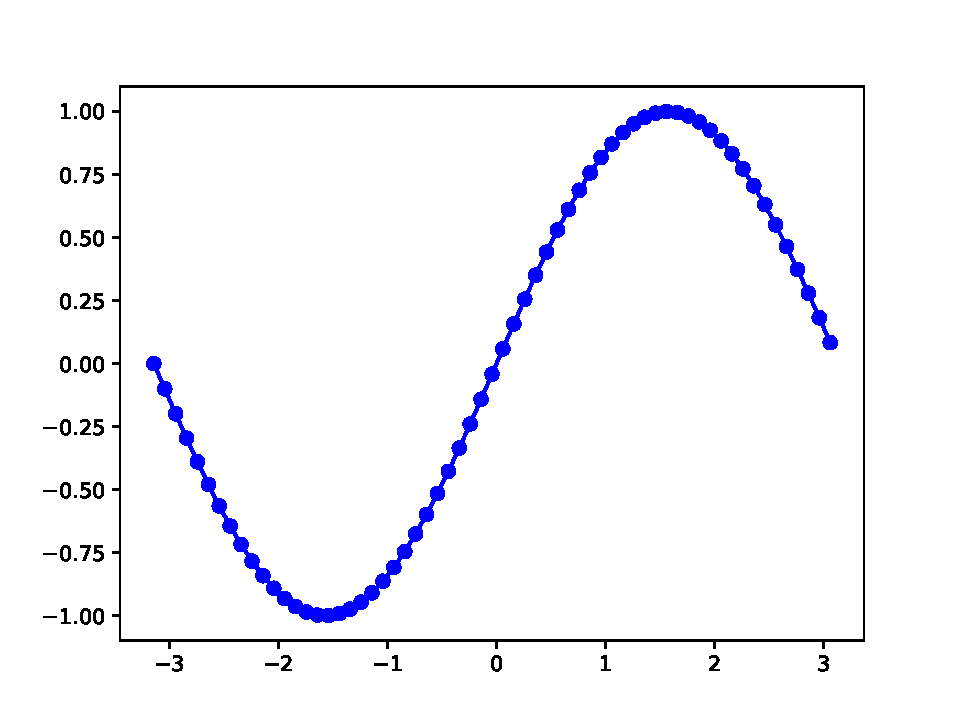
\includegraphics[scale=0.7]{fig/sinx.pdf}
    \caption{ソースコード\ref{matplot1}の出力結果}
    \label{fig:sinx}
\end{figure}

\begin{table}[H]
    \centering
    \caption{主な線の種類}
    \begin{tabular}{c|c}
        \hline
        スクリプト上での記号 & 線の種類 \\
        \hline\hline
        \texttt{-} & 実線 \\
        \texttt{--} & 破線 \\
        \texttt{-.} & 一点鎖線 \\
        \texttt{:} & 点線 \\
        \hline
    \end{tabular}
    \label{tab:linestyle}
\end{table}

\begin{table}[H]
    \centering
    \caption{主なマーカーの種類}
    \begin{tabular}{c|c}
        \hline
        スクリプト上での記号 & 線の種類\\
        \hline\hline
        \texttt{.} & 点 \\
        \texttt{,} & ピクセル \\
        \texttt{o} & 丸 \\
        \texttt{\^} & 三角 \\
        \texttt{v} & 下三角 \\
        \texttt{<} & 左三角 \\
        \texttt{>} & 右三角 \\
        \texttt{s} & 四角 \\
        \texttt{d} & 菱形 \\
        \texttt{+} & $+$ \\
        \texttt{x} & $\times$ \\
        \hline
    \end{tabular}
    \label{tab:marker}
\end{table}

\begin{table}[H]
    \centering
    \caption{主な色の種類}
    \begin{tabular}{c|c}
        \hline
        スクリプト上での記号 & 色\\
        \hline\hline
        \texttt{r} & 赤 \\
        \texttt{g} & 緑 \\
        \texttt{b} & 青 \\
        \texttt{c} & シアン \\
        \texttt{m} & マゼンタ \\
        \texttt{y} & 黄 \\
        \texttt{k} & 黒 \\
        \texttt{w} & 白 \\
        \hline
    \end{tabular}
    \label{tab:color}
\end{table}

\end{document}
